\documentclass[tikz,border=2pt]{standalone}
\usepackage{xcolor}
\usepackage{pgfplots}
\usetikzlibrary{arrows.meta}

\pgfplotsset{compat=1.16}
\pgfplotsset{
  singlebarlegend/.style={
    legend image code/.code={
      \draw[##1] (0cm,-0.08cm) rectangle (0.25cm,0.08cm);
    }
  }
}

\definecolor{paperBlue}{RGB}{55,96,146}
\definecolor{paperTeal}{RGB}{74,135,126}
\definecolor{paperGold}{RGB}{190,137,48}
\definecolor{paperRed}{RGB}{164,78,76}
\definecolor{paperGray}{RGB}{92,92,92}

\begin{document}
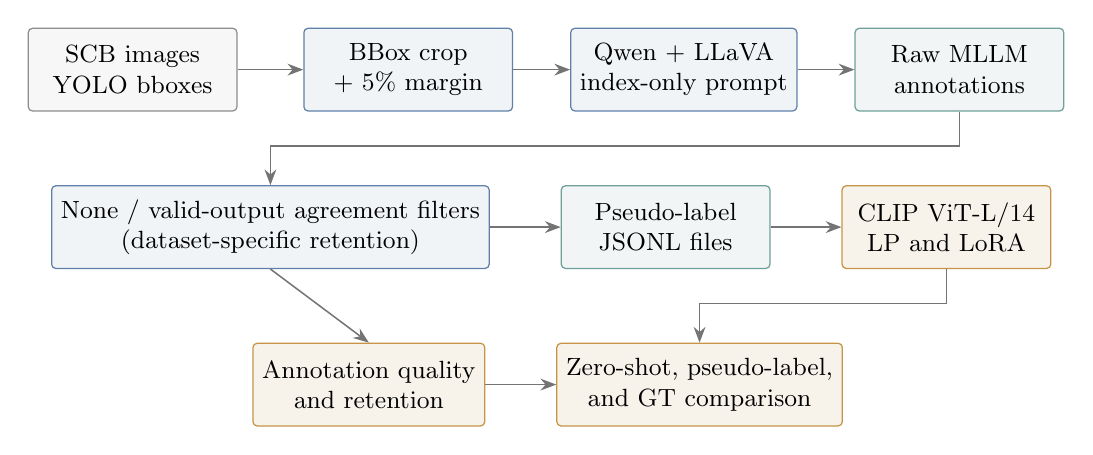
\begin{tikzpicture}[
  font=\small,
  box/.style={draw=paperGray!70, line width=0.45pt, rounded corners=1.5pt,
              align=center, minimum width=2.65cm, minimum height=1.05cm,
              fill=black!3},
  proc/.style={draw=paperBlue!80, line width=0.45pt, rounded corners=1.5pt,
              align=center, minimum width=2.65cm, minimum height=1.05cm,
              fill=paperBlue!7},
  outbox/.style={draw=paperTeal!80, line width=0.45pt, rounded corners=1.5pt,
              align=center, minimum width=2.65cm, minimum height=1.05cm,
              fill=paperTeal!8},
  eval/.style={draw=paperGold!90, line width=0.45pt, rounded corners=1.5pt,
              align=center, minimum width=2.65cm, minimum height=1.05cm,
              fill=paperGold!10},
  arrow/.style={-{Stealth[length=2mm]}, line width=0.55pt, draw=paperGray!85}
]
\node[box]  (data) at (0,0) {SCB images\\YOLO bboxes};
\node[proc] (crop) at (3.5,0) {BBox crop\\+ 5\% margin};
\node[proc] (mllm) at (7.0,0) {Qwen + LLaVA\\index-only prompt};
\node[outbox]  (ann)  at (10.5,0) {Raw MLLM\\annotations};

\node[proc] (filter) at (1.75,-2.0) {None / valid-output\/ agreement filters\\(dataset-specific retention)};
\node[outbox, anchor=west]  (pseudo) at ([xshift=9mm]filter.east) {Pseudo-label\\JSONL files};
\node[eval, anchor=west] (clip) at ([xshift=9mm]pseudo.east) {CLIP ViT-L/14\\LP and LoRA};

\node[eval] (diag) at (3.0,-4.0) {Annotation quality\\and retention};
\node[eval, anchor=west] (result) at ([xshift=9mm]diag.east) {Zero-shot, pseudo-label,\\and GT comparison};

\draw[arrow] (data.east) -- (crop.west);
\draw[arrow] (crop.east) -- (mllm.west);
\draw[arrow] (mllm.east) -- (ann.west);
\draw[arrow] (ann.south) |- ([yshift=5mm]filter.north) -- (filter.north);
\draw[arrow] (filter.east) -- (pseudo.west);
\draw[arrow] (pseudo.east) -- (clip.west);
\draw[arrow] (filter.south) -- (diag.north);
\draw[arrow] (clip.south) |- ([yshift=5mm]result.north) -- (result.north);
\draw[arrow] (diag.east) -- (result.west);
\end{tikzpicture}
\end{document}